

\subsection*{Задача по критерию Неймана-Пирсона}

Производится однократно измерение количества сработавших ячеек SiPM. Известно, что оно распределено по закону Пуассна $p(k, \lambda)$. 
% светить зеленым лазером в чай/сою
Нулевая гипотеза $H_0$: $\sub{\lambda}{dark} = 14$. 

Найдём пороговое значение $k_b$: $\alpha = 5 \times  10^{-6}$:
\begin{equation*}
    \int_{k_b}^{\infty} \frac{\sub{\lambda}{dark}^k}{k!} e^{-\sub{\lambda}{dark}} \d k = 
    \left\{\begin{aligned}
        &7.0 \times 10^{-6}, &k_b = 33; \\
        &2.8 \times 10^{-6}, &k_b = 34,
    \end{aligned}\right.
\end{equation*}
откуда можем сказать, что $k_b > 33$ -- подходит. Более точное значение $\alpha = 5.0 \times  10^{-6}$будет достигаться при  $k_b = 33.375$.
% ашкен, нобелевская премия по стрикции. 

Найдём теперь подходящее для $\beta = 0.9$ значение $S$:
\begin{equation*}
    \beta = \int_{0}^{k_b} p(k,\, \sub{\lambda}{dark} + S) \d k,
    \hspace{0.5cm} \Rightarrow \hspace{0.5cm}
    1-\beta = \left\{\begin{aligned}
        &0.91, &S=28; \\
        &0.89, &S=27,
    \end{aligned}\right.
\end{equation*}
откуда находим $S = 28$.

\begin{figure}[h]
    \centering
    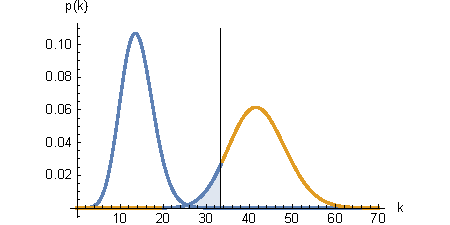
\includegraphics[width=0.5\textwidth]{mrc.pdf}
    \caption{Распределения для $\sub{\lambda}{dark}$ и $\sub{\lambda}{dark} + S$.}
    %\label{fig:}
\end{figure}




\subsection*{Задача про два пучка}

Пучок расходится под углом $\lambda/d$, тогда эффективная можность упадет в $(\lambda/d)^2$. Така как число квантов совпадает, то можем считать
\begin{equation*}
    N \sim \left(\frac{\lambda}{d}\right)^{-2} \frac{h c}{\lambda} \sim \frac{1}{\lambda^3},
    \hspace{0.5cm} \Rightarrow \hspace{0.5cm}
    \frac{N_1}{N_2} = \left(\frac{\lambda_2}{\lambda_1}\right)^3 =  10^{15},
\end{equation*}
где $\lambda_2 = 10$ см,  $\lambda_1 = 1\ \mu$м.